
\documentclass{article} \title{Report Labwork 3: Hello CUDA} 
\usepackage{graphicx}
\author{Nguyen Huy Hung} 
\date{\today} 
\begin{document} 
\maketitle {Mage image RGB-to-gray converter using CUDA}
\section{CPU} 
In this labwork, my main environment runtime is using Google Colab.
Firstly, Loading image from file by using matplotlib library. After that, we will flat image into 1D array of RGB. For each row now will represent one pixel (R, G, B).
In using CPU with for range, we use the simple formula to convert to gray is gray = (red + green + blue)/3. 
So here will be steps to use: 

1. Allocate gray scale: Creates a flat array to hold gray scales pixel values.

2. Loop over each pixel using for range: Using formula to compute their average and assign it to array

3. Reshape back to image: Convert back to image shape
\begin{figure}[h]
    \centering
    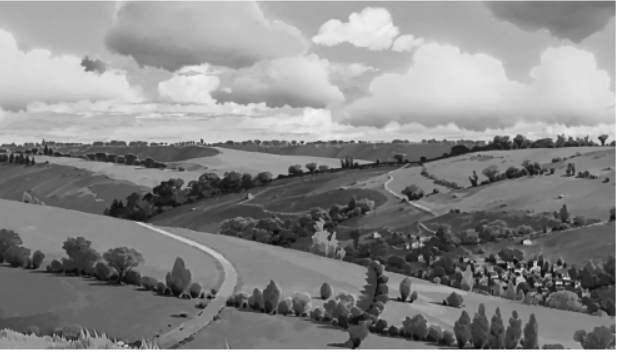
\includegraphics[width=0.7\textwidth]{E:/advancedhpc2025/LABWORK3/Gray-sample.png}
    \caption{Sample grayscale image}
    \label{fig:gray-sample}
\end{figure}
\section{GPU}
In this section, we follow do but not using CPU, we will use GPU to convert RGB image to gray.
So the pipeline for it will be: 

1. Host feeds device with data

2. Host ask device to process data

3. Device processes data in parallel

4. Device return result

Gpu will need data to process. So first we need copy data to GPU. Using .todevice() function to do it. 
Next we will need to define CUDA kernel:
 
@cuda.jit

def rgb2grayflat(img, gray, totalpixel):

    i = cuda.grid(1)

    if i < totalpixel:

        r = img[i, 0]

        g = img[i, 1]

        b = img[i, 2]

        gray[i] = (r + g + b) / 3

Each CUDA thread will process exactly one pixel. CUDA organizes work in blocks and threads. In here i create each block has 256 threads. next is grid, which i want to be enough blocks for cover all pixels.
blockspergrid = (totalpixel + threadsperblock - 1) // threadsperblock.

After done configure GPU execution, we will launch kernel and copy result back to CPU.
\section{Experimenting with different block size values}

For experiment, we will try to test block size with 6 sizes to compare about execution time. The size includes: 32, 64, 128, 256, 512, 1024.
After do the same step for each sizes, we get the result is: 

Block size 32: 0.407424 ms

Block size 64: 0.183200 ms

Block size 128: 0.147456 ms

Block size 256: 0.143360 ms

Block size 512: 0.166528 ms

Block size 1024: 0.441088 ms

In here, we can see that we have good performance when block sizee is 128 and 256. When size block is small like 32 or 64, the execution time quite slow. But when threads is more like 512 or 1024, the performance is dropped.
It could be because of  scheduling ineffeciency.
\begin{figure}[h]
    \centering
    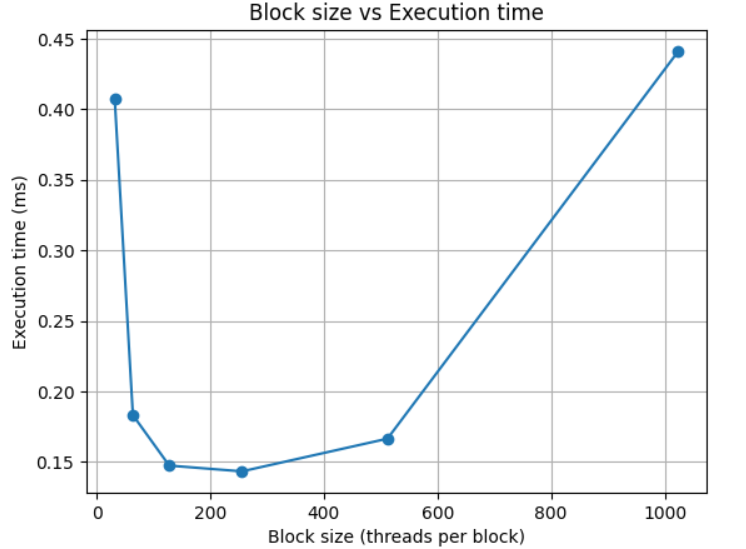
\includegraphics[width=0.7\textwidth]{E:/advancedhpc2025/LABWORK3/Exp.png}
    \caption{Experiment about block size}
    \label{fig:gray-sample}
\end{figure}

\end{document}